\section{The enigma of Gamma Ray Bursts}
\label{sec:enigma}
Humans have long explored the universe beyond the `visible' wavelengths. From the low-frequency radio waves used to detect cosmic microwave background radiation, to the high-frequency ``hard'' X-rays and $\gamma$-rays\footnote{The distinction between ``soft'' and ``hard'' X-rays, as well as ``hard X-rays'' and ``$\gamma$-rays,'' is subjective, and loose. In this Thesis, photons of energies less than $10$ keV will be referred to as ``soft X-rays,'' photons of energies between $10$ keV and $200$ keV will be referred to as ``hard X-rays,'' and those with larger energies will be referred to as ``$\gamma$-rays.''},  they have opened their eyes to observe the universe in all domains of the electromagnetic spectrum. Each new window has initially thrown up mysteries, clouding the vision until years of effort cleared it. Recently, we have opened up a set of `ears': gravitational waves [GWs].

Just as necessity has driven invention, war has pushed the frontiers of human knowledge to expedite discoveries otherwise unlikely, if not impossible. One such discovery is what we know today as `Gamma Ray Bursts' [GRBs]. In the height of the Cold War, the American `Vela' satellites, while playing vigil to possible violations of the Nuclear Test Ban Treaty by the erstwhile U.S.S.R, chanced upon a phenomenon that remained shrouded in mystery as classified government documents until its astrophysical nature was firmly established. Reported $5$ years since discovery \citep{Klebesadel_et_al.-1973-ApJL}, Gamma Ray Bursts remained an enigma for another two decades.

As the name suggests, GRBs are `bursts' of $\gamma$-rays: short-lived, transient phenomenon in the hard X-ray/$\gamma$-ray detectors, lasting from milliseconds to tens of seconds. $\gamma$-ray photons are absorbed by the Earth's atmosphere, hence making life possible, but requiring observation from above the atmosphere. On the other hand, these high-energy photons pass with ease through detector materials. This necessitates increasing the area of the detecting material to register more photons, compromising on the sky-localisation of the X-ray/$\gamma$-ray sources. This meant that the sky localisation of the bursts was very poor, covering hundreds of square degrees. Unable to tell whether these astrophysical sources originated in our own galaxy [the Milky Way] or not, plausible theories included everything above and beyond the earth, colliding neutron stars to giant flares on our Sun [see \cite{Nemiroff-1994-review} for a review].

In the years following the discovery, GRBs remained a mystery primarily due to the lack of association with other astrophysical objects. To do this, one required the sky location of the burst to follow up at other wavelengths, but that had to be done before the burst faded. Although the InterPlanetary Network [IPN] \citep{Cline_and_Desai-1976-Ap&SS} was set up in the 1970s and provided localisation of some bursts up to a few hundred square degrees, it was still a large part of the sky for ground-based optical/infrared telescopes to attempt a follow-up. Moreover, the delay from the detection to the localisation was much more than the burst time-scales, and hence they could not be followed up.

It was only in the 1990s when the $\gamma$-ray detector Burst And Transient Alert Telescope [\B] \citep{Fishman_et_al.-1989-BAAS} on-board the \emph{Compton Gamma Ray Observatory} [\emph{CGRO}] started detecting GRBs routinely, and localising them to degrees accuracy \citep{Briggs-1995-Ap&SS}, that their isotropic distribution on the sky was firmly established. Still the debate between extragalactic distances and sources distributed in the Milky Way halo, remained, urgently requiring an estimation of the distance. With significant technological advancements of the Italian-Dutch satellite \bs\ \citep{Boella_et_al.-1997-A&AS}, GRBs could be followed up at larger wavelengths at a few hours' times-scales, and the redshift measurement of two GRBs by identifying the host galaxies, GRB970228 \citep{van_Paradijs_et_al.-1997-Nature} and GRB970508 \citep{Metzger_et_al.-1997-Nature}, firmly established that they were located at cosmological distances.

The cosmological locations of GRBs raised more questions than answers. Given their large distances, short durations, and the observed flux, their intrinsic luminosities [$\sim 10^{52} \, \ergpersec$] were orders of magnitude greater than any astrophysical object ever known: they outshine their entire parent galaxies in the short lifespan, the brightest supernova by around $10$ orders of magnitude, and even the more powerful distant quasars by at least $3$ orders of magnitudes. What powers them? The clue lay in the fact that not a single GRB was ever found to repeat, indicating that they were signatures of cataclysmic events, possibly violent deaths of massive stars. Given the finite speed of light, their short time-scales implied that the length-scales associated with them are much smaller than astronomical length-scales, indicating that they were associated with compact objects, like neutron stars [NSs] and black holes [BHs].


\section{What we know about GRBs}
\label{sec:what_we_know}
We have come a long way since the discovery of GRBs, and the age of the enigma of GRBs is over. Today, we can claim to understand GRBs as well as we understand BHs. Questions remain unanswered, but we are not hunting in the dark.

The quantity used to define the duration of a burst is called the $\T$, defined as the interval in which the central $90 \%$ of the flux is observed. Based on the observed distributions of $\T$\footnote{and `hardness', a measure of whether more photons were detected in a larger energy window, as compared to a smaller energy window} of a sample of GRBs detected by \B, \cite{Kouveliotou_et_al.-1993-ApJ} [hereafter \citetalias{Kouveliotou_et_al.-1993-ApJ}] found that the sample can be divided into the so-called `long' and `short' bursts, $\T \lessgtr 2$ s. The observed event rate was found to be $\sim 150 \, \py$ on an average for `long GRBs' [LGRBs], and $\sim 10 \, \py$ for `short GRBs' [SGRBs], almost an order of magnitude smaller. Over the years, several lines of evidence suggested that the two classes are physically distinct classes, having different progenitors. Being associated with Type Ic supernovae \citep{Woosley_and_Bloom-2006-ARA&A} and also exclusively located at star forming regions within their galaxies \citep{Wainwright_et_al.-2007-ApJ, Fruchter_et_al.-2006-Nature}, LGRBs were conclusively associated with the death of massive stars collapsing directly into black holes \citep{MacFayden_and_Woosley-1999-ApJ, Woosley_and_MacFayden-1999-A&AS}. On the other hand, the lack of supernovae associations with SGRBs, their occurrence in older and elliptical galaxies, large offset from the host galaxy, etc. [see \cite{Berger-2014-sGRB_review} for a review] suggested that the SGRB progenitor is the merger of compact objects, like a pair of neutron stars [NSs], or a NS-BH, giving rise to relativistic jets \citep{Eichler_et_al.-1989-Nature, Narayan_et_al.-1992-ApJ} [also see \cite{Nakar-2007-PhR} for a review]. Recently, the detection of gravitational waves [GWs] from a binary neutron star merger [BNSM], GW170817 \citep{GW170817-2017}, along with its electromagnetic counterparts including the predicted `kilonova' \citep{EM170817-2017}, provided conclusive evidence of this association.

Irrespective of the differences of the progenitors, the `central engine', that is the source of energy that powers the transient emission is similar for the two classes of GRBs \citep{Ghirlanda_et_al.-2009-A&A, Calderone_et_al.-2015-MNRAS}: ultra-relativistic jets powered from the immediate environment of the nascent NS or BH [see \cite{Kumar_and_Zhang-2015-PhR} for a detailed review]. The Lorentz factors of these jets can be as high as $1000$ at the start of the prompt emission phases \citep{Abdo_et_al.-2009-Science}. The primary questions regarding GRBs can be posed in terms of questions regarding the launching and composition of the relativistic jets that give rise to the prompt emission. The physics of highly relativistic plasma in the presence of high magnetic fields, is however not extremely well-understood. Only recently has extensive computer simulations being catching up with the myriad details of non-thermal emission from ultra-relativistic matter originating very close to a nascent NS or BH, taking into account the effects of general relativity as well as three-dimensional hydrodynamics \citep{Sasha_et_al.-2008-MNRAS, Sasha_et_Al.-2010-NewA, Narayan_et_al.-2011-MNRAS}.

Observational distinction is made between the `prompt' emission phase, that is the short-lived X-ray/$\gamma$-ray emission, and the progressively longer time-scale emission observed at smaller frequencies lasting for hours, even days to weeks in the radio wavelengths. This so-called `afterglow' emission was understood to be arising from the circumbust medium of the GRB progenitors: as the relativistic jets entrain the circumbust medium and drive shocks through it, they slow down, and the circumbust medium cools down at progressively smaller frequencies at larger distances from the centre of the progenitor. The evidence of the `achromatic jet-break' \citep{Fruchter_et_al.-1999-ApJ, Kulkarni_et_al.-1999-Nature, Stanek_et_al.-1999-ApJ, Harrison_et_al.-1999-ApJ, Frail_et_al.-2001-ApJ} [also see \cite{Fong_et_al.-2012-ApJ}, \cite{Fong_et_al.-2015-ApJ} for a summary] that is, the sudden drop in flux during the afterglow, proved to the smoking-gun evidence that the jets are ultra-relativistic, the jet-break being a direct consequence of the relativistic Doppler beaming. The reader is referred to \cite{Kumar_and_Zhang-2015-PhR} for a recent, extremely detailed review of the observations and theory of afterglow emission.

Studying the afterglow emission tells us about the environment of the GRB progenitors, as well as the large-scale properties of the jet. On the other hand, the prompt emission arises from ultra-relativistic matter very close to the newly-formed NS or BH. Hence, a careful study of the timing, spectroscopy, and polarization of the unprocessed hard X-ray and $\gamma$-ray prompt emission offers an unique probe to the launching and composition of relativistic jets from regions very close to compact objects.

There are broadly two kinds of research done with GRBs. From the early days of observation, it was known that each GRB has a timing profile, called the ``lightcurves,'' different from all others. Just like snowflakes, each GRB is unique. The first kind of research attempts to answer generic questions of the physics of relativistic jets -- their launching, composition, energy-scales, etc. -- via detailed studies of individual GRBs. This requires not only detection of GRBs, but also following them up individually with larger wavelength pointing telescopes, which can facilitate the identification of the host-galaxy. This, in turn, can help in estimating the distance to the burst, offer insights into the GRB formation process via their positions within the host galaxies, and help us study the chemical properties of the burst environment. The identification of the host galaxy of the first binary neutron star merger event GW/EM 170817 \citep{GW170817-2017, EM170817-2017} showed the importance of being able to do this kind of research.

The second kind of research done tries to use the fact that GRBs are seen at very large distances in the universe due to the extremely high luminosities. For example, \cite{Cucchiara_et_al.-2011-ApJ} reported the detection of GRB090429B at a redshift of $9.4$, at $\sim 5\%$ of the age of the present age of the universe, the most distant GRB seen till date. Studying populations of GRBs can offer insights into the way GRBs have formed through cosmic time-scales, the evolution of galaxies, etc. Claims have been made to use GRBs as an addition to the cosmic distance ladder \citepalias{Tan_et_al.-2013-ApJL}. But as we shall see in this Thesis, research along these lines lets us make important contributions to the study of individual GRBs.



\section{GRBs and \AS-CZTI}
\label{sec:GRBs_and_AstroSat}
The current dedicated GRB monitors in space are \s\ \citep{Gehrels_et_al.-2004-ApJ} and \f\ \citep{FermiGBM-2009-ApJ}, launched in 2004 and 2008 respectively. \s\ observes only a tenth of the sky, and detects a GRB once in every $\sim 3$ days. Its triggering instrument is called the Burst Alert Telescope [BAT], which is sensitive to only the hard X-rays, from $15$ to $150$ keV. It uses an imaging technique with the help of the coded aperture mask [CAM] on-board BAT \citep{Band-2006-ApJ} to localise the detected GRB within a small region of the sky and slew to this location within roughly a minute, providing even more precise localisation with its softer X-ray and ultraviolet detectors, which are then followed up by ground-based detectors to study the afterglow emission \citep{Barthelmy_et_al.-2005-SSRv-SwiftBAT}. Living up to its name, it has increased the number of GRBs with afterglow observations. \f\ on the other hand is an open detector, virtually observing the full sky, and is also sensitive within a wide range of $8$ keV to $10$ MeV. It detects [on an average] one GRB per day, but can provide only rough localisation of the detected GRB, which is a large patch in the sky [about tens of square degrees]. Hence, unlike \s, it does not facilitate the detection of afterglows.

\AS\ is an Indian multi-wavelength satellite, simultaneously observing a wide range of the electromagnetic spectrum: from optical/ultraviolet to hard X-rays/$\gamma$-rays \citep{Rao_et_al.-2016-arXiv-Astrosat}. It has four instruments on-board: Ultra-Violet Imaging Telescope [UVIT] \citep{Subramaniam_et_al.-2016-SPIE, Tandon_et_al.-2017-AJ, Tandon_et_al.-2017-JApA, Rahna_et_al.-2017-MNRAS}, Soft X-ray Telescope [SXT] \citep{Singh_et_al.-2016-SPIE, Singh_et_al.-2017-JApA}, Large Area X-ray Proportional Counter [LAXPC] \citep{Agrawal_et_al.-2017-JApA, Antia_et_al.-2017-ApJS, Yadav_et_al.-2017-arXiv}, and Cadmium Zinc Telluride Imager [CZTI] \citep{Bhalerao_et_al.-2017-JApA}. CZTI is a hard X-ray detector sensitive in the energy range $20$-$400$ keV, consisting of an array of CdZnTe crystals. Each detector module consists of $256$ independent detectors, called `pixels,' of size $2.5$ mm $\times \; 2.5$ mm each. The detector plane consists of four quadrants, each with $16$ detector modules, comprising an effective area of $1024 \, \rm{cm{^2}}$. CZTI has imaging capabilities below $100$ keV, using the Coded Aperture Mask [CAM] placed above collimator slats that surround the detector modules. The collimator is made of Tantalum of size $4$ cm $\times$ $4$ cm, which allows for a field of view [FOV] of $4.6^{\circ} \times 4.6^{\circ}$.

\begin{figure}
\begin{center}
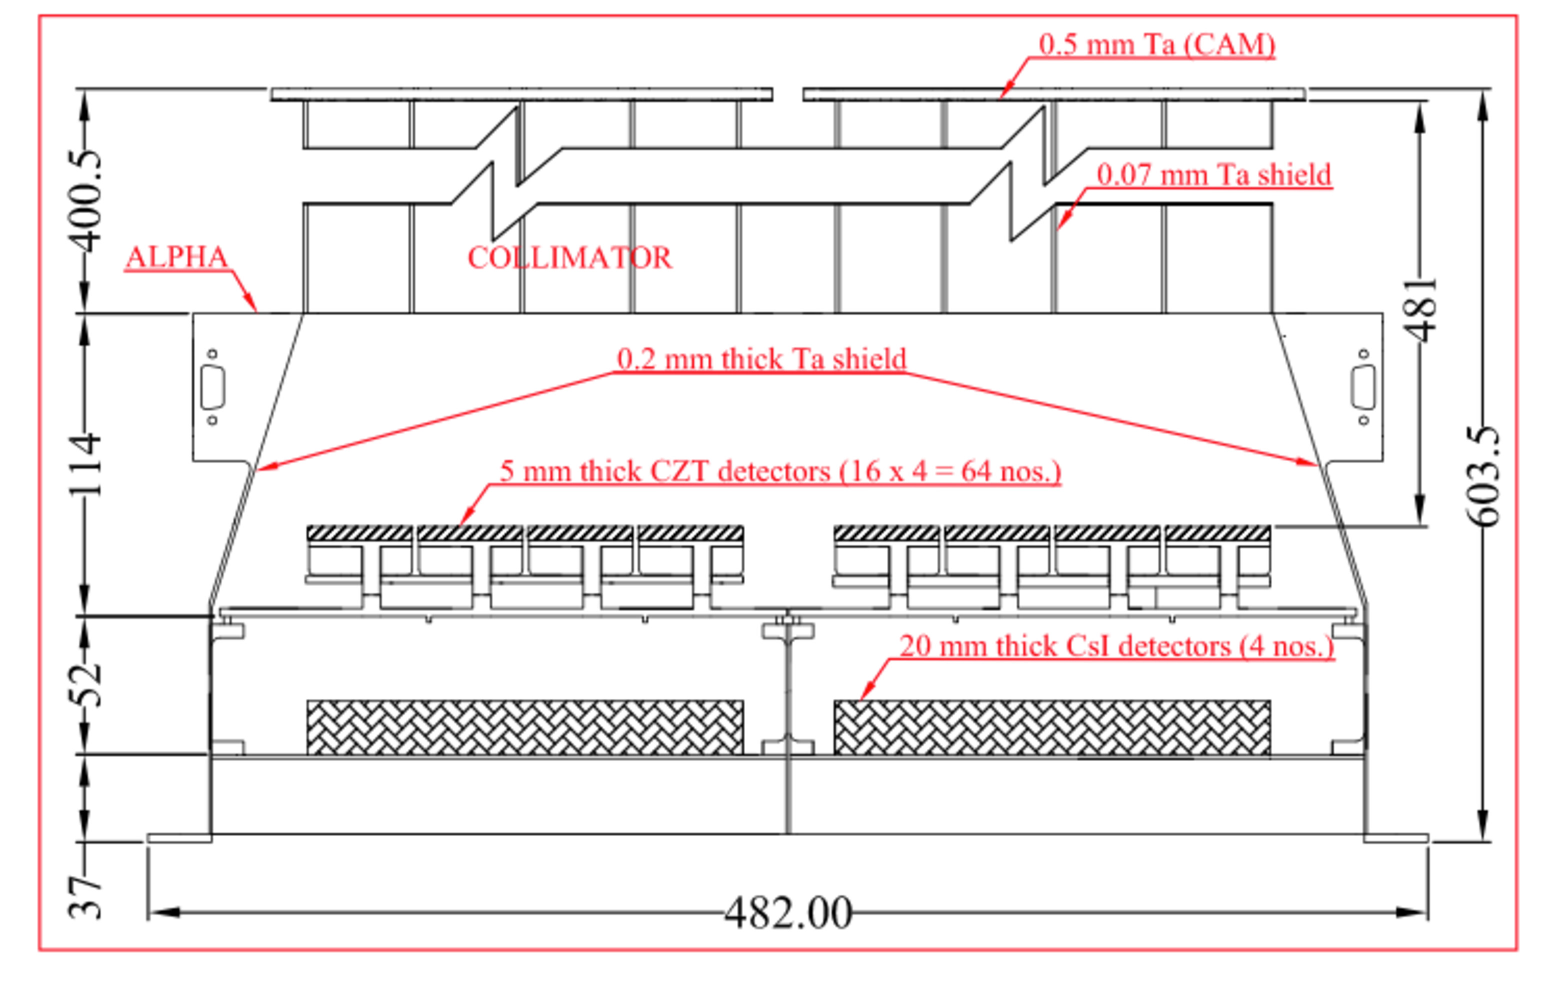
\includegraphics[scale=0.33]{GRB151006A--CZT}
\caption[Schematic diagram of \AS -CZTI]{A schematic diagram of the CZT instrument on the \AS\ satellite. All dimensions are in millimeters. A Tantalum coded aperture mask [CAM] at the top is backed by $400$ mm Al/Ta collimators, which restrict the view to $4.6^{\circ} \times 4.6^{\circ}$. Four identical quadrants with arrays of thick CZT modules forms the focal plane, $481$ mm below the CAM. The $2.46$ mm pixels matched to the CAM pitch provide a native angular resolution of $\sim 17^{'}$ in the primary field of view. $20$ mm thick CsI(Tl) scintillators mounted $\sim 66$ mm below the CZT modules provide active anti-coincidence shielding, and also function as a wide-angle detector in the $100$-$500$ keV range. Courtesy: \cite{Rao_et_al.-2016-ApJ}.}
\label{fig:CZTI}
\end{center}
\end{figure}

After \AS\ was launched on the 28\textsuperscript{th} September, 2015, CZTI was the first payload to start observing astrophysical sources, on the 6\textsuperscript{th} October, 2015. On the very same day, it detected a long duration Gamma Ray Burst [GRB]: GRB151006A, which was also detected by \s\ and \f\ [the nomenclature refers to the date of detection by the \s\ satellite]. \s\ provided accurate sky-localisation, and \f\ provided a wide-band spectrum. This was the golden opportunity to calibrate \AS -CZTI. Using this GRB, it was shown in \cite{Rao_et_al.-2016-ApJ} that CZTI has capabilities of: (1) accurate timing studies of sources via time-tagged photon data every $20 \, \mus$; (2) spectroscopy in the wide range of hard X-rays via channel-to-energy conversion of the individual photons; (3) polarization studies of bright sources via the informations of detector-position and energy of coincident photons; and (4) few degrees localisation of transients detected off-axis, detailed in Chapter \ref{chap:localisation}.

Complementing the capabilities of the softer energy mission \s\ [$15$-$150$ keV] which has an unique capability of following up GRBs in real-time, and the harder energy mission \f\ [$8$ keV-$10$ MeV] which can accurately study the evolution of the spectra of the GRBs, CZTI was seen to possess the exciting capabilities of studying the unprocessed X-ray emission from GRBs at energy-range in-between \s\ and \f, as well as provide additional polarisation constraints. \cite{Basak_et_al.-2017-MNRAS} used the combined capabilities of \AS -CZTI along with the \s\ and \f\ data for this GRB to infer the re-injection of energy in the jet at $\sim 16$-$20$ s from the start of the prompt emission, even though the pulse profile was smooth throughout its activity.

\AS -CZTI has continued to play a crucial role in the study of GRBs ever since its inception. \cite{Chand_et_al.-2018-ApJ} reported high polarization from GRB 160802A, and used CZTI's capability of simultaneous temporal,  spectral, and polarimetric studies to infer about the emission mechanism of this GRB, as well as the properties of its jet. \cite{Chattopadhyay_et_al.-2017-arXiv} reported polarisation from $11$ GRBs in the first two years of \AS 's operation. This significantly increasing the number of GRBs with polarisation measurements, which can be used to constrain the emission mechanism of GRBs in general. \cite{Bhalerao_et_al.-2017-ApJ-A_Tale_of_Two_Transients} investigated whether the gravitational wave [GW] source GW170104 \citep{GW170104-2017}, a BH-BH binary, was associated with any electromagnetic counterpart. They reported the non-detection of any electromagnetic transient, and concluded that the GRB170105A detected by \AS -CZTI but not by \s\ or \f,  happened to be more than $20$ hours after GW170104, and was just a regular long GRB. Upon the first detection of an electromagnetic counterpart to a GW source GW170817 \citep{GW170817-2017, EM170817-2017}, \AS -CZTI played a crucial role via its non-detection of GRB170817A, detected by \f: It was understood that this source was in the Earth's shadow of CZTI, otherwise it would be detected with a signal-to-noise [SNR] of $> 10$, which information was used to rule out a large part of the sky for the localisation of this source \citep{Kasliwal_et_al.-2017-Science}.

\section{Scope of this Thesis}
\label{sec:scope}
In view of exciting studies of Gamma Ray Bursts using \AS -CZTI, one question becomes important to answer: What is the number of GRBs that \AS -CZTI can detect in a given time? The answer depends both on the instrumental characteristics of \AS -CZTI, as well as the intrinsic population of both long and short GRBs. There exists a true all-sky rate of GRBs, accounting for their cosmological rate of formation. A GRB detector samples from this superset, depending on its characteristics: solid angle of observation, average run time, the energy-band at which it observes, its flux-limit [also referred to as the `sensitivity'], etc. Hence, if the true cosmological and intrinsic distribution of GRBs can be theoretically constructed, one should be able to recover the rate of GRB detections by any X-ray/$\gamma$-ray detector, by specifying the detector's characteristics. As a by-product, one would also be able to study the intrinsic properties of the populations of both long and short bursts. With firm empirical evidence of the association of BNSMs and SGRBs, one may similarly ask: What is the rate of BNSMs that the current and future GW detectors are likely to detect? The answer lies in a careful study of the population of SGRBs.

Consider the following situation: There exists a population of torches at different distances from the observer. If all the torches had the same luminosity, then all torches up to a certain distance would be observed, whereas others at distances larger than that would not be. This limiting distance would be defined by the flux-limit of the observing instrument. But what if the torches had different luminosities? Then this intrinsic distribution over the parameter space of the torches' luminosities, written as $L$, would have to be taken into account to predict the number of torches we could observe with the same instrument. So is the case with GRBs and GRB detectors in space. The `luminosity function' [LF] is a probabilistic distribution function over the luminosity of the entire population of GRBs, denoted by $\Phi (L)$. To calculate the expected GRB-detection rate of \AS, it becomes necessary to construct this detector-independent quantity, separately for long and short GRBs. This Thesis reports the most updated constraints on the luminosity function of the long GRBs in Chapter \ref{chap:LGRBs}, and short GRBs in Chapter \ref{chap:SGRBs}. These are then used to predict the detection-rate of LGRBs and SGRBs for \AS -CZTI, as well as other future X-ray/$\gamma$-ray missions. These predictions are topical, and helps plan mission operations well in advance, as demonstrated in both these chapters.

Upon tallying the number of GRBs that \AS -CZTI actually detects versus the numbers predicted, it is noticed that a significant fraction of GRBs is missing. In Chapter \ref{chap:noise}, the reason behind this is carefully highlighted, via a re-investigation of the data analysis pipeline currently in place. Previously unreported in the CZTI data, high energy cosmic rays are detected. It is shown that the presence of this component in the data increases the number of false-positives of possible transients, to eliminate which, a significant number of GRBs are missed. A novel approach to solve this problem is proposed, and is currently being integrated in the CZTI data-analysis pipeline.

GRB photons are known to be powered by relativistic particles in large-scale collimated jets, via non-thermal mechanisms like synchrotron emission. The angular dependence of the non-thermal emission plays an important role in how the true cosmological population of GRBs is observed by an earth-based detector [Chapters \ref{chap:LGRBs} and \ref{chap:SGRBs}]. Hence, it is important to theoretically predict the angular dependence of synchrotron emission from relativistic jets. In Chapter \ref{chap:jet_model}, this was carried out in the more simple quasi-static regime, that is, when the particle distribution in the jet is quasi-statically maintained by the central engine. The formulae derived can be extended to GRBs by keeping the parameters of the model functions of time. The time-scale of evolution of these parameters will then be the time-scale of energy-injection by the central engine. The full-scale application of this idea is the scope of future work.

No scientific venture is ever complete: as one question is answered, new questions emerge. As an extension of comparing the durations of GRBs detected both by \s\ and by \f\ carried out in Chapter \ref{chap:LGRBs}, a careful re-investigation of this common catalogue of GRBs revealed a significant discrepancy of the durations of a small subset of bursts. To figure out the reason, each of these GRBs are being currently studied, and the preliminary idea and directed efforts are briefly summarised in Chapter \ref{chap:ongoing}. Finally, concluding remarks are presented in Chapter \ref{chap:conclusions}.

All the codes contributing to this Thesis were written in the free programming language, \textsc{python}, using freely available standard libraries. In line with the idea of open research, the codes have been made publicly available except to avoid conflicts with collaboration protocols.